\documentclass[tikz, border=2mm]{standalone}
\usetikzlibrary{shapes, arrows.meta}

\begin{document}

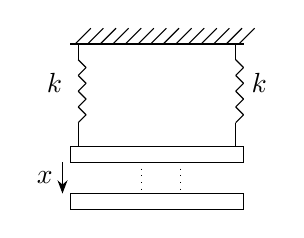
\begin{tikzpicture}
    % Support rod (horizontal)
    \draw (0.4,2) -- (2.6,2); % Shortened the support system
    
    % First Rectangle
    \draw (0.4,0.5) rectangle (2.6,0.7); % Centered the first rectangle
    
    % First Spring (tight rod)
\draw (0.5,1.8) -- (0.5,2);
    \draw (0.5,1.8) -- (0.6,1.7);
    \draw (0.6,1.7) -- (0.5,1.6);
    \draw (0.5,1.6) -- (0.6,1.5);
    \draw (0.6,1.5) -- (0.5,1.4);
    \draw (0.5,1.4) -- (0.6,1.3);
    \draw (.6,1.3) -- (0.5,1.2);
    \draw (0.5,1.2) -- (.6,1.1);
    \draw (.6,1.1) -- (0.5,1);
    \draw (0.5,1)--(0.5,0.7);
    \node at (0.2, 1.5) {$k$};
    
    % Second Rectangle (dotted)
    \draw (0.4,0.1) rectangle (2.6,-0.1);
    
    % Second Spring (tight rod)
    \draw (2.5,1.8) -- (2.5,2);
    \draw (2.5,1.8) -- (2.6,1.7);
    \draw (2.6,1.7) -- (2.5,1.6);
    \draw (2.5,1.6) -- (2.6,1.5);
    \draw (2.6,1.5) -- (2.5,1.4);
    \draw (2.5,1.4) -- (2.6,1.3);
    \draw (2.6,1.3) -- (2.5,1.2);
    \draw (02.5,1.2) -- (2.6,1.1);
    \draw (2.6,1.1) -- (02.5,1);
    \draw (02.5,1)--(02.5,0.7);
    \node at (2.8, 1.5) {$k$};
    
    \foreach \i in {1,...,14}
        \draw ({0.3 + 0.16*\i},2) -- ({0.5 + 0.16*\i},2.2);
    
    \draw[thin, dotted] (1.3,0.5) -- (1.3,0.1);
    \draw[thin, dotted] (1.8,0.5) -- (1.8,0.1);
    
    % Arrow downwards for \delta x
    \draw[->, >=Stealth] (0.3, 0.5) -- node[midway, left] {\(x\)} (0.3, 0.1);
\end{tikzpicture}

\end{document}

